\subsubsection{\textit{Overfitting}}\label{overfitting}

Sabiendo el funcionamiento básico de una red neuronal usando el algoritmo de \textit{feed-forward} y \textit{backpropagation} se puede pensar que si en cada iteración del modelo, la red entrena y aprende nuevos patrones, se puede sacar la conclusión de que realizando un entrenamiento infinito se puede obtener un modelo perfecto cuyo el error se ha minimizado lo máximo posible y por lo tanto los resultados esperados son los esperados. Pero esto no es así, tener una configuración errónea de la red o entrenar a la red más debidamente de lo necesario provoca lo que es conocido como \textit{overfitting}.
\newline

El \textit{overfitting} es un problema bien conocido a la hora de entrenar redes neuronales. En español, significa sobreajustado y suele ser causa de usar un entrenamiento que se ha realizado por mucho tiempo, provocando que el modelo se ajuste perfectamente a los datos de entrenamiento y de algún modo “memorice” los datos y por lo tanto, no sepa extrapolar y adaptarse a otros casos. En otras palabras, se sobreajustan la matrices $W$ de todas las capas y así, el modelo se adapta perfectamente a los datos de entrada produciendo que el modelo no sea capaz de estimar un valor correcto cuando se usa un vector de entrada que antes no lo había visto.

\begin{figure}[H]
    \centering
    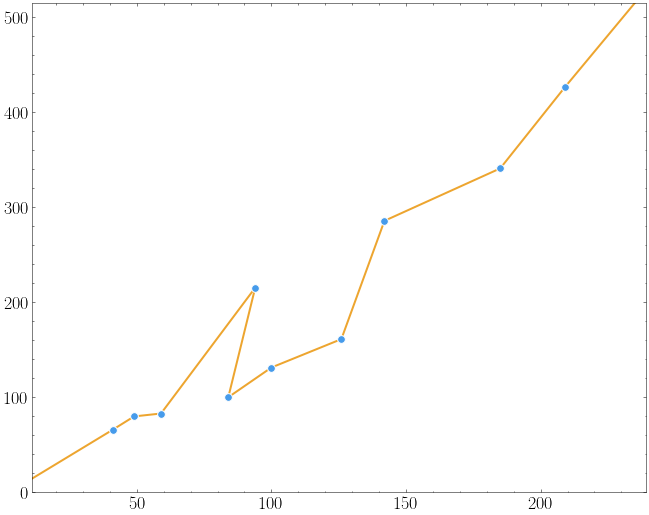
\includegraphics[width=12cm]{images/state-of-art/overfitting/overfitting.png}
    \caption{Ejemplo de \textit{overfitting} en una regresión lineal.}
    \label{fig:basic_network}
\end{figure}

manteniendo la precisión de los datos de prueba mientras nuestra red se entrena. 

Una de las maneras más rápidas de saber si un modelo se está entrenando con \textit{overfitting} es usando un segundo dataset además del de entrenamiento. Normalmente, antes de crear una red neuronal hay que realizar un preprocesado de datos explicadas en la Sección TODO. Como bien se explica en esa sección, el dataset original se suele dividir en tres dataset distintos: entrenamiento, validación y test. Obviamente, el \textit{dataset} de entrenamiento es usado para entrenar e ir ajustando los parámetros de las matrices $W$ de forma iterativa. Por otro lado, se tiene los \textit{datasets} de validación y test que son usados para evaluar distintas métricas. Si el problema que se quiere resolver con la red es de tipo regresión se suele usar como métrica algún tipo de error explicados en la Sección \ref{costfunction} como por ejemplo: \textit{MAE}, \textit{MSE} o error de \textit{Huber}. Por otro lado si el problema a resolver es de clasificación, se suele usar la precisión como métrica.
\newline

Si vemos que la precisión de los datos de prueba ya no mejora, entonces deberíamos dejar de entrenar. Por supuesto, en sentido estricto, esto no es necesariamente un signo de \textit{overfitting}. Podría ser que la precisión de los datos de la prueba y los datos de entrenamiento dejen de mejorar al mismo tiempo. Aún así, la adopción de esta estrategia evitará el exceso de adaptación.
\newline

Al finalizar de cada \textit{epoch}, se usarán un subconjunto de datos del \textit{dataset} de entrenamiento y otro subconjunto del \textit{dataset} de validación. Con ellos, se calculará el valor de la métrica seleccionada y se obtendran dos valores. Estos valores se puede comparar entre ellos. Dos valores que son parecidos indican que el modelo es capaz de estrapolar a otros casos que no ha usado para el entramiento. Por el contrario, si el valor asociado al \textit{dataset} de entrenamiento es mucho mejor que el asociado al de validación esto puede significar que el modelo pueda estar sufriendo de \textit{overfitting}. Un entrenamiento llevado a cabo sin \textit{overfitting} se puede visualizar en la figura TODO.
\newline

Al inicio del entrenamiento, como la red no ha sido entrenada y los paramétros inicializados aleatoriamente, el modelo tendrá unas métricas bastantes malos, es decir, si se está usando algún error, dicho valor será muy alto. Por otro lado si se está midiendo la precisión del modelo dicho valor distará mucho del 100\%. Estas métricas serán igualmente malas tanto para ambos \textit{datasets}. Según vayan ocurriendo \textit{epochs} en el entrenamiento, llegará un momento que el modelo no pueda mejorar más y comenzará a memorizar los datos con los que esta siendo entrenado del \textit{dataset} de entrenamiento provocando que la métrica asociada al entrenamiento sea casi perfecta y la de validación progresivamente vaya empeorando. Un ejemplo de un entremiento que sufre de \textit{overfitting} puede verse de la siguiente manera:
\newline

\begin{figure}[H]
    \centering
    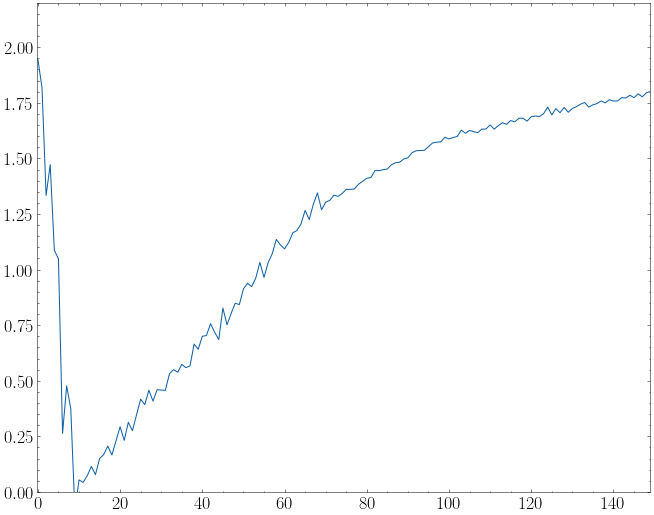
\includegraphics[width=12cm]{images/state-of-art/overfitting/overfitting-loss.png}
    \caption{Ejemplo de \textit{overfitting} en una regresión lineal usando un error como métrica.}
    \label{fig:basic_network}
\end{figure}

Al comienzo del entrenamiento ambas métricas van en pararelo, hasta que llegan a la \textit{epoch} X, en ese punto se puede visualizar como la métrica de validación poco a poco va empeorando. Es en ese punto donde se ve que la red tiene un problema de \textit{overfitting}. Dependiendo de la métrica usada, el \textit{overfitting} puede aparecer antes o después, pero es un tema más complejo que no se explicará en este trabajo.
\newline

Aún así hay varias técnicas que se explicarán a continuación para evitar el \textit{overfitting}: 
\begin{itemize}
    \item Regularización L1 y L2:
    Son dos métodos que calculan un valor conocido como penalización que se añade al error y de ese modo poder penalizar parámetros con valores grandes. Si una neurona tiene valores grandes puede ser signo de que la neurona está intentando memorizar. De hecho, se considera una mala práctica dejar que un conjunto pequeño de neuronas de la red sean las que más responsabilidad tengan, es decir, que sus parámetros asociados sean muy grandes.
    \newline
    
    Por un lado, se tiene L1 que es la suma de todos los valores absolutos de $w$ y $b$. Es una penalización linear ya que la función asociada es directamente proporcional a los parámetros. La penalización L2 es la suma de todos los parámetros $w$ y $b$ al cuadrado. Es una función no lineal y penaliza con mayor intensidad a os valores grande a diferencia de L1 que penaliza mucho más en proporción a los valores pequeños por ser lineal. Esto causa que el modelo empieza a ser invariante a pequeños valores de entrada y variante solo a los valores grandes. Por ello, L1 es raramente usado a nor ser que sea en combinación con L2. Ambas funciones están en función de un valor $\lambda$, con este valor se puede dictar cuanto impacto tendrá L1 y L2 en el error final. Matemáticamente:
    
    \begin{align*}
         L_{1w} = \lambda \sum_m |w_m| &&  L_{2w} = \lambda \sum_m w^2_m \addtocounter{equation}{1}\tag{\theequation} \\ 
         L_{1b} =\lambda \sum_n |b_n| && L_{2b} = \lambda \sum_n b^2_n \addtocounter{equation}{1}\tag{\theequation}
    \end{align*}
    

    El error final viene dado por la simple suma del error calculado por la función de coste y L1 con L2:
    \begin{equation}
        c_T = c + L_{1w} + L_{1b} + L_{2w} + L_{2b}
    \end{equation}
    
    Como se usa la regularización para el calculo de $c$, hace falta saber su derivada para poder usar el \textit{back-propagation}. Quedando la derivada de coste de la siguiente forma:
    
    \begin{equation}
        \frac{\partial c_T}{\partial w^{L_i}} = c' + L'_{1w} + L'_{1b} + L'_{2w} + L'_{2b}
    \end{equation}
    
    Las derivadas de L1 y L2 son las siguientes:
    \begin{align*}
         L'_{1w} = \lambda \begin{cases} 1,& \text{si } w_m > 1\\ -1,& \text{si } w_m < 1\end{cases} && L'_{2w} =  2\lambda w_m \addtocounter{equation}{1}\tag{\theequation} \\ 
         L'_{1b} =  \lambda \begin{cases} 1,& \text{si } b_n > 1\\ -1,& \text{si } b_n < 1\end{cases} && L'_{2b} = 2\lambda b_n \addtocounter{equation}{1}\tag{\theequation}
    \end{align*}
    
    \item \textit{Dropout} \label{dropout}: Usando esta técnica, en cada iteración del entrenamiento la red se modifica. Supongamos que se tiene un \textit{input} $x$ y el valor deseado $y$. Ordinariamente, se entrenaría mediante la propagación hacia adelante de $x$ a través de la red, y luego la propagación hacia atrás para determinar la contribución al gradiente. Con \textit{dropout}, este proceso se modifica. Se comienza eliminando aleatoriamente (y temporalmente) un porcentaje de las neuronas ocultas en la red, mientras que se deja las neuronas de entrada y salida sin modificar. Las neuronas que han sido borradas, serán neuronas "fantasmas" para ese \textit{epoch}:
    
    \begin{figure}[H]
        \centering
        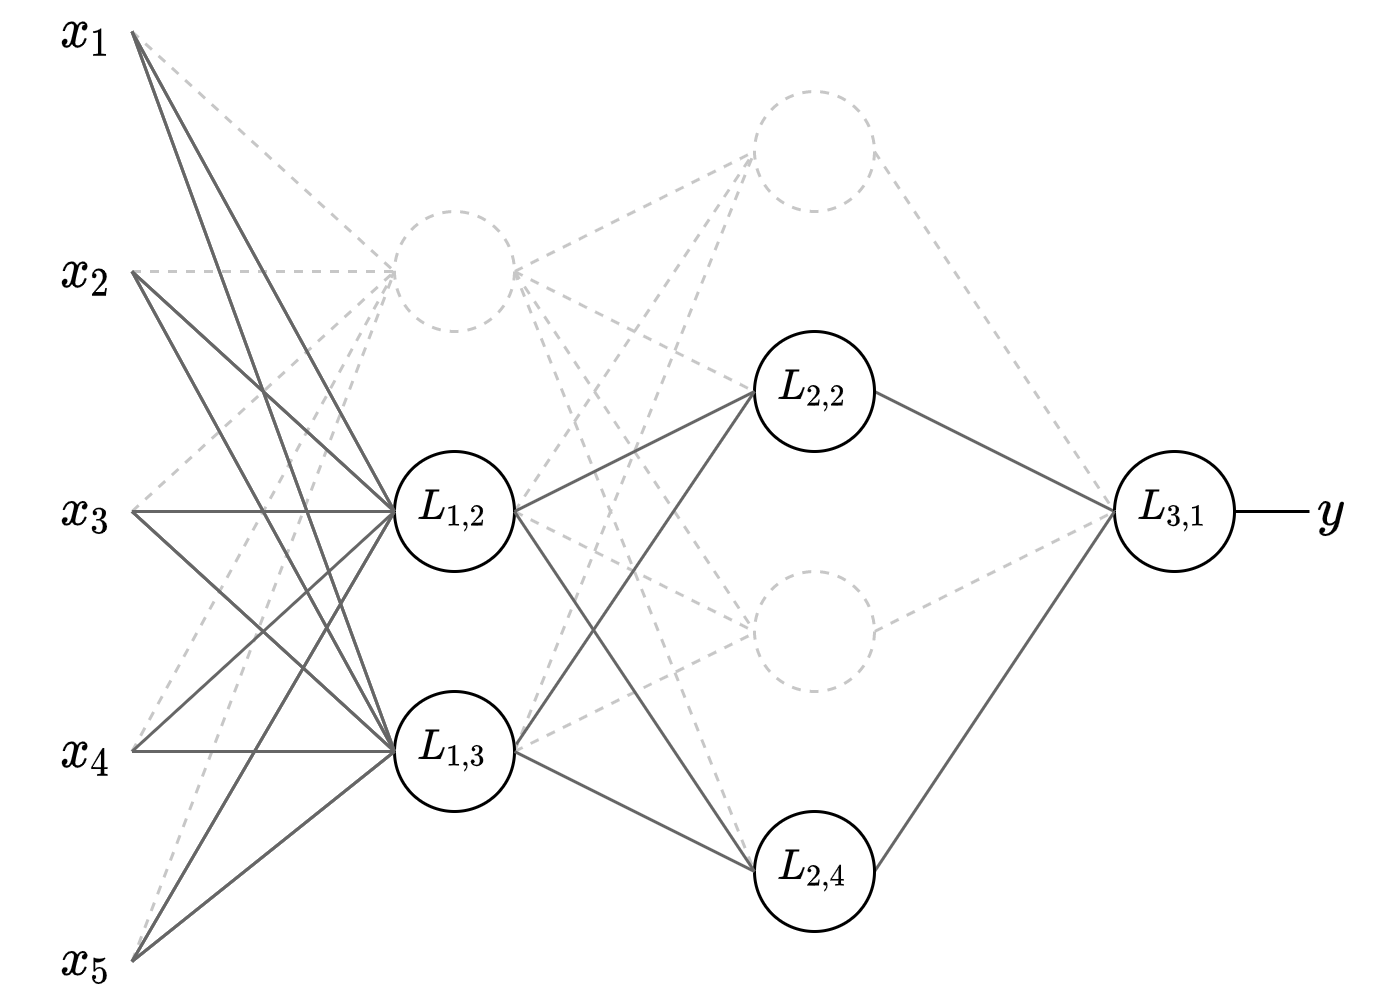
\includegraphics[width=12cm]{images/state-of-art/overfitting/dropout-1.png}
        \caption{\textit{Dropout} aplicado a una red con un $50\%$  de probabilidades}
        \label{fig:basic_network}
    \end{figure}
    
    Una vez terminado el proceso de propagación hacia adelante y \textit{backpropagation}, se comenzará un nuevo \textit{epoch} eliminando aleatoriamente un conjunto de neuronas. Es resumen, por cada iteración, se eliminar un subconjunto de las neuronas de acuerdo a un porcentaje dado.
    \newline
    
    Repitiendo este proceso durante toda la fase de entrenamiento, la red aprenderá unas matrices $W$ que se habrán aprendido en condiciones en las que un subconjunto de las neuronas ocultas fueron eliminadas. Cuando realmente se ejecuta la red completa, significará que el número de neuronas activas será mayor. Por ello, se compensar reduciendo la parte proporcional con las que fueron entradas. Por ejemplo, usando un porcentaje igual a $50$, los valores de $W$ serán la mitad de lo que el gradiente haya calculado.
    

\end{itemize}

% Curse of dimensionalrity
%TODO Ejemplo de modelo normal vs modelo con overffiting

% L1 and L2 regularization
